\section{CUARTA SECCIÓN}

\lipsum[20]

A continuación, se presentan tablas con los parámetros que definen al comportamiento histerético bilineal para edificaciones con aislamiento de base con diferentes razones de aislamiento ($r=T_{M}/T_{f}$). 

\begin{table}[!ht]
\centering
\vspace{1.5 mm}
\caption[Parámetros de la interfaz de aislamiento $r=2$]{\centering\footnotesize Parámetros de la interfaz de aislamiento $r=2$}
\vspace{1 mm}
\begin{tabular}{|c|c|M {1.25 cm}|M {1.25 cm}|M {1.25 cm}|M {1.25 cm}|M {1.25 cm}|M {1.25 cm}|}
\hline
\multirow{2}{*}{Símbolo} & \multicolumn{1}{l|}{\multirow{2}{*}{Unidad}} & \multicolumn{6}{c|}{Número de Niveles}      \\ \cline{3-8} 
                         & \multicolumn{1}{l|}{}                        & $n=3$    & $n=6$    & $n=9$   & $n=12$  & $n=15$  & $n=18$  \\ \hline
$T_{f}$                  & $s$                                          & 0.30   & 0.60   & 0.90  & 1.20  & 1.50  & 1.80  \\ \hline
$Q^{*}$                  & $g$                                          & 0.191  & 0.095  & 0.064 & 0.047 & 0.030 & 0.022 \\ \hline
$K_{p}^{*}$              & $1/s^{2}$                                    & 75.16  & 18.79  & 8.51  & 4.70  & 3.01  & 2.19  \\ \hline
$K_{e}^{*}$              & $1/s^{2}$                                    & 751.59 & 187.90 & 85.12 & 46.97 & 30.06 & 21.91 \\ \hline
\end{tabular}
\label{Ca3_Tabla4}
\end{table}


	\subsection{Importancia de la Razón de Aislamiento}
	
	\lipsum[29]
	
	\begin{figure}[!h]
	\centering
		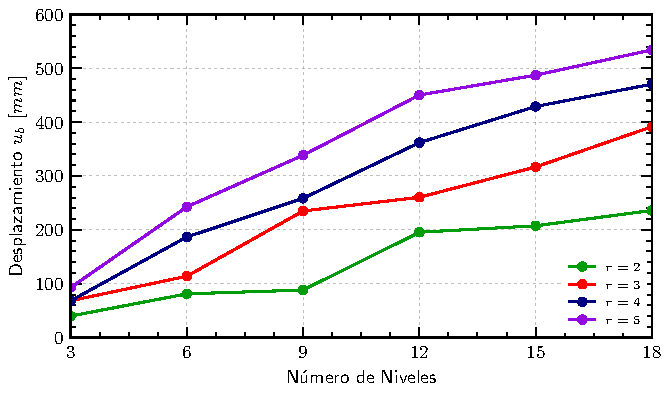
\includegraphics[scale=1]{E_IMAGENES/1_Capitulo3/Cap3_Imagen9.pdf}
		\vspace{-3 mm}
	\caption[Desplazamiento máximo de la interfaz de aislamiento]{\centering\footnotesize Desplazamiento máximo de la interfaz de aislamiento.}
	\label{Cap3_Figura9}
	\end{figure}

